
\todo{write uberleitung}

\begin{defin}
    Let $\B$ be a colored braided operad. We call $\B$ \emph{representable} if
    it fulfills the following: For every finite set $I$, $I$-labeled
    configuration $\widetilde{I}$, collection of colors $\{X_i\}_{i \in I}$
    there is a \emph{representing color}
    \[
    \bigotimes_{i \in \widetilde{I}} X_i
    \]
    with a \emph{representing morphism}
    \[
    f \in \Mul_{\B}^{\widetilde{I}}\left(\left\{X_i\right\}_{i \in I}, \bigotimes_{i \in \widetilde{I}} X_i\right)
    \]
    such that the following universal property holds: Let $Y$ be a color in
    $\B$. Then for all $I$-labeled configurations $\widetilde{I}'$ and $g \in
    \Mul_{\B}^{\widetilde{I}'}(\{X_i\}_{i \in I}, Y)$ there exists a unique

    $$\bar{g} \in \Mul_{\B}^{\id^{(1)}}\left(\left\{\bigotimes_{i \in
    \widetilde{I}} X_i\right\}, Y\right)$$
    \todo{one unique morph for all paths or for a path we find one unique? then choice of path relevant! }
    such that for a composition map $\gamma$ corresponding to any path $\eta$:
    \begin{center}
        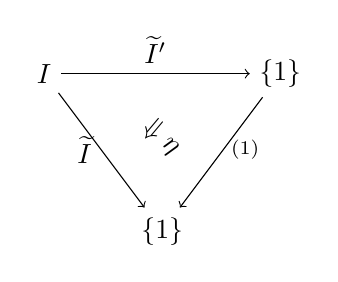
\begin{tikzpicture}
            % Define node positions
            \node (B) at (0, 2) {$I$}; \node (C) at (3, 2) {$\{ 1 \}$}; \node
            (A) at (1.5, 0) {$\{ 1 \}$};
            
            % Draw arrows
            \draw[->] (B) -- (C) node[midway, above] {$\widetilde{I}'$};
            \draw[->] (B) -- (A) node[midway, left] {$\widetilde{I}$}; \draw[->]
            (C) -- (A) node[midway, right] {$\id^{(1)}$};
            
            % Natural transformation arrow
            \node[rotate=-40] at (1.5, 1.2) {$\Downarrow \eta$};
            % \node at (1.7, 1.2) {$\eta$};
        \end{tikzpicture}
    \end{center}
    it hold:
    \[
        g = \gamma(f, \bar{g})
    \]
\end{defin}

This definition yields a braided monoidal structure on the underlying category
of a colored braided operad $\B$.

\begin{const}\label{con:braidmon} Let $\B$ be a representable colored braided
    operad. We denote the underlying category by $\C$ and define
    \[
        \otimes \colon \C \times \C \to \C
    \]
    to be the functor that maps
    \[
        (X_1,X_2) \mapsto \bigotimes_{i \in b_2} X_i
    \]
    where  $\bigotimes_{i \in b_2} X_i$ is representing color of $\{X_i\}_{1,2}$
    with $b_2$ denoting the basepoint configuration in $\E_2(2)$ being a
    $\langle 2 \rangle^{\circ}$-configuration:
    
    \begin{center}
    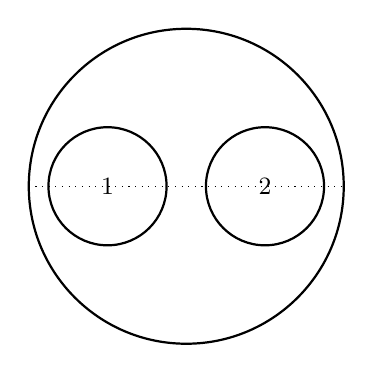
\begin{tikzpicture}
                        % First element (left)
                        \node at (1, 0) {\small $2$}; \node at (-1, 0) {\small
                        $1$};
                        
                        \draw[thick] (0,0) circle (2); \draw[thick] (1, 0)
                        circle (0.75); \draw[thick] (-1, 0) circle (0.75);
                        \draw[dotted](-2, 0)--(2, 0);       
        \end{tikzpicture}
    \end{center}

    While for morphisms
    \[
        h \in \Mul_{\B}^{\id^{(1)}}\left(\{X_1\}, X_1'\right) \; \text{and} \;  g \in \Mul_{\B}^{\id^{(1)}}\left(\{X_2\}, X_2'\right)
    \] 
    and representing morphisms 
    \[
    f \in \Mul_{\B}^{\id^{(1)}}\left(\left\{X_i\right\}_{1 \leq
    i \leq 2}, \bigotimes_{i \in b_2} X_i\right) \; \text{and} \; f' \in
    \Mul_{\B}^{\id^{(1)}}\left(\left\{X_i'\right\}_{1 \leq i \leq 2},
    \bigotimes_{i \in b_2} X_i'\right),
    \]
    we obtain $\gamma(h,g,f')$ and by the universal property of $f$ we get a
    unique morphism:
    \[
        h \otimes g \in \Mul_{\B}^{\id^{(1)}}\left(\left\{\bigotimes_{i \in b_2} X_i\right\}, \bigotimes_{i \in b_2} X_i'\right)
    \]
    such that $\gamma(f, h \otimes g) = \gamma(h,g,f')$. 
    

    For $h = \id_{X_1}$ and $g=\id_{X_2}$ and $f \in
    \Mul_{\B}^{\id^{(1)}}\left(\left\{X_i\right\}_{1 \leq i \leq 2},
    \bigotimes_{i \in b_2} X_i\right)$, then there is $\id_{X_1} \otimes
    \id_{X_1}$ such that $\gamma(f, \id_{X_1} \otimes \id_{X_1}) = f$. Further,
    we observe
    \[
        \gamma(f,\id_{\bigotimes_{i \in b_2} X_i}) = f
    \]
    Due to uniqueness, we must have
    \[
        \id_{X_1} \otimes \id_{X_1} = \id_{\bigotimes_{i \in b_2} X_i}.
    \]
    As for the composition, let $h \in \Mul_{\B}^{\id^{(1)}}\left(\{X_1\},
    X_1'\right)$, $h' \in \Mul_{\B}^{\id^{(1)}}\left(\{X_1'\}, X_1''\right)$, $g
    \in \Mul_{\B}^{\id^{(1)}}\left(\{X_2\}, X_2'\right)$, $g' \in
    \Mul_{\B}^{\id^{(1)}}\left(\{X_2'\}, X_2''\right)$

    and
    \begin{align*}
        f \in \Mul_{\B}^{\id^{(1)}}\left(\left\{X_i\right\}_{1 \leq i \leq 2},
    \bigotimes_{i \in b_2} X_i\right) \\
    f' \in \Mul_{\B}^{\id^{(1)}}\left(\left\{X_i'\right\}_{1 \leq i \leq 2},
    \bigotimes_{i \in b_2} X_i'\right) \\
    f'' \in \Mul_{\B}^{\id^{(1)}}\left(\left\{X_i''\right\}_{1 \leq i \leq 2},
    \bigotimes_{i \in b_2} X_i'\right)
    \end{align*}
    for which the following hold:
    \begin{align}%
        \gamma(f, \gamma(h,h') \otimes \gamma(g,g')) &= \gamma(\gamma(h,h'), \gamma(g,g'), f'') \label{eq:representable1}\\
        \gamma(f', h' \otimes g') &= \gamma(h',g',f'') \label{eq:representable2}\\
        \gamma(f, h \otimes g) &= \gamma(h,g,f') \label{eq:representable3}
    \end{align}
    Let us consider the following calculation using associativity in $\B$ and
    the above equations:
    \begin{align*}
        \gamma\left(f, \gamma(h \otimes g, h' \otimes g')\right) &= \gamma(\gamma(f, h \otimes g), h' \otimes g') \\
        & \overset{\eqref{eq:representable3}}{=} \gamma(\gamma(h,g,f'), h' \otimes g') \\ 
        & = \gamma(\gamma(h,g, \gamma(f', h' \otimes g'))) \\
        & \overset{\eqref{eq:representable2}}{=}   \gamma(\gamma(h,g,\gamma(h',g',f''))) \\
        & = \gamma(\gamma(h,h'), \gamma(g,g'), f'') 
    \end{align*}

    From this calculation we see that equation \eqref{eq:representable1} also holds for $\gamma(h
    \otimes g, h' \otimes g')$. Due to uniqueness by the universal property of
    $f$, it follows:
    \[
        \gamma(h,h') \otimes \gamma(g,g') = \gamma(h \otimes g, h' \otimes g')
    \]
    Thus, $\otimes$ is indeed a well-defined functor.
    

    Let $\beta$ denote the following morphism in $\Br$
     \begin{align*}
         \beta \colon \langle 2 \rangle^{\circ} &\to \langle 2 \rangle^{\circ} \\
         1 &\mapsto 2 \\
         2 &\mapsto 1 \\
     \end{align*}
    with the collection $(\id^{(2)}, \id^{(1)})$. We denote the basepoint
    configuration with permuted labels by $\beta(b_2)$, as it corresponds to the
    composition
    \[
     \langle 2 \rangle^{\circ} \overset{\beta}{\to} \langle 2 \rangle^{\circ} \overset{b_2}{\to} \langle 1 \rangle^{\circ}.
    \]

    Let $\{X_i\}_{i=1,2}$ be a collection of colors. For configurations $b_2$
    and $\beta(b_2)$ we obtain:
    \[
        \bigotimes_{i \in b_2} X_i ;\ \text{and} ;\ \bigotimes_{i \in \beta(b_2)} X_i
    \]
    with representing morphisms $f$ and $f^{\beta}$ respectively. Then, by the
    universal property of $f$ we obtain for $f^{\beta}$, $\bigotimes_{i \in
    \beta(b_2)} X_i$ and the half twist $\htw$:
    \begin{center}
    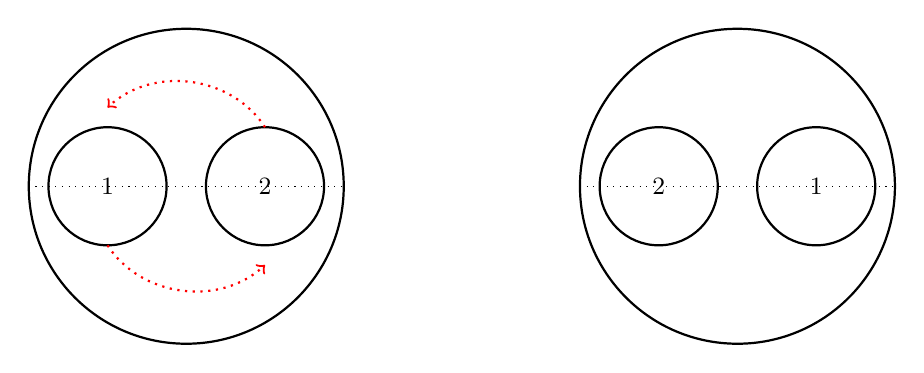
\begin{tikzpicture}
                        % basepoint
                        \node at (1, 0) {\small $2$}; \node at (-1, 0) {\small
                        $1$};
                        
                        \draw[thick] (0,0) circle (2); \draw[thick] (1, 0)
                        circle (0.75); \draw[thick] (-1, 0) circle (0.75);
                        \draw[dotted](-2, 0)--(2, 0); \draw[->, thick, dotted,
                        red] (-1, -0.75) to [bend right=50] (1, -1); \draw[->,
                        thick, dotted, red] (1, 0.75) to [bend right=50] (-1,
                        1);

                        \node at (3.5, 0) {$\rightsquigarrow$};
                        
                        % twisted basepoint
                        \node at (8, 0) {\small $1$}; \node at (6, 0) {\small
                        $2$};
                        
                        \draw[thick] (7,0) circle (2); \draw[thick] (8, 0)
                        circle (0.75); \draw[thick] (6, 0) circle (0.75);
                        \draw[dotted](5, 0)--(9, 0);  
                        
        \end{tikzpicture}
    \end{center}
    A unique morphism
    \[
        b \in \Mul^{\id^{(1)}}_{\B}\left(\bigotimes_{i \in b_2} X_i, \bigotimes_{i \in \beta(b_2)} X_i \right).
    \]
    Vice versa, from the universal property of $f^{\beta}$ we gain for $f$,
    $\bigotimes_{i \in b_2} X_i$ and the inverse half twist $\htw^{-1}$ a unique
    morphism:
    \[
        b^{-1} \in \Mul^{\id^{(1)}}_{\B}\left(\bigotimes_{i \in \beta(b_2)} X_i, \bigotimes_{i \in b_2} X_i \right).
    \]
    These morphisms are indeed inverse to one another: It holds that:
    \[
        f^{\beta} = \gamma(f, b), ;\ f=\gamma(f^{\beta}, b^{-1})
    \]
    Further, the identiy is the unique morphism for the unique lift for the
    representable morphisms itself with the trivial path. Thus,
    \[
        \gamma(b^{-1}, b) = \id_{\bigotimes_{i \in \beta(b_2)}X_i},  \; \gamma(b, b^{-1}) = \id_{\bigotimes_{i \in b_2}X_i}.
    \]
    This, defines a natural isomorphism. The monoidal unit is defined by the
    representing color of the empty collection $\{\}$ with the empty
    configuration which we denote by $\mathbf{1}$. The associator is defined as
    follows:
    \todo{associator missing}
    \todo{argument why applying $\otimes$ twice results in $\tau_1^3$ object}
\end{const}

\begin{cla}
    Let $\B$ be a representable colored braided operad and $\C$ denoting its
    underlying category. Then the Construction \ref{con:braidmon} defines a
    braided monoidal structure on $\C$.
\end{cla}

We will not give a proof of the claim. However, the arguments used to verify
unitality, pentagon and hexagon identities are similar to the proof given for
Proposition \ref{prop:braidmon}.

For a representable colored braided operad $\B$, we claim that the braided
monoidal structure from Construction \ref{con:braidmon} coincides with the
braided monoidal structure we gain from the forgetful functor $\Bx \to \Brx$
given in Construction \ref{con:brx_monoidal}. In fact, we claim that the
representation property of a colored braided operad induces a co-fibration on the
forgetful functor. This however would need addition work. If the forgetful functor
is an op-fibration, it is somewhat straightforward to show that the colored braided operad is representable
as a cocartesian morphism over $\langle n \rangle \to \langle 1 \rangle$
is a representing morphism.




